\section{Methodology}\label{sec:method}
In this section, we elaborate on the symbolic reasoning framework for some common feed-forward network verification tasks with $\ell_p$-perturbations. These are considered as the standard DNN verification problems. %This demonstrates how we apply the framework on the standard problem. %We will additionally show that the power of symbolic reasoning, especially compared with abstract-interpretation-based methods, on reasoning recurrent structures. 
We first present an overview of the symbolic reasoning framework, and then show how we can concretely apply this framework to verify DNNs in different scenarios.

\subsection{Overview}\label{sec:overview}
Similar to the classical symbolic execution~\cite{symbex}, the framework ``executes'' the DNN and generates an optimization program that precisely characterizes the problem of interest\footnote{We categorize the satisfiability program as an optimization program in this paper. For example, it is easy to transform a SAT problem into a MaxSAT problem.}. For this step, the challenge is how we can execute the DNN symbolically and also encodes the verification problem that we aim to address. We utilize the expressiveness of quadratic relations, and the resulting program is a QP rather than a satisfiability program in the classical symbolic execution.

In the classical symbolic execution, once the satisfiability program is generated, one can use off-the-shelf solvers such as the SMT solver to solve the program~\cite{smt}. Our framework contains an extra relaxation step to achieve \emph{efficiency}. Many DNN verification tasks are known $\NP$ or $\coNP$-hard~\cite{reluplex,IUA,geolip}. Because the QPs exactly encode the problems of interest, they are also hard to solve. However, we want to address the verification problem efficiently, i.e., in polynomial time, so we need to relax the QP. We use Shor's relaxation scheme, to transform the hard-to-solve QP to the convex SDP. SDPs can be solved efficiently both theoretically and in practice.

\paragraph{Neural-network execution}A feed-forward network is a composition of affine transformations and non-linear activations. To reason it symbolically, we associate symbols with the input and the output of any component function, and then relate those symbols with quadratic relations. See~\cref{fig:network} for an example.

Therefore, we only need to symbolically execute the affine transformation and the activation function. For affine transformations, it is straightforward because affine relations are linear and so quadratic. The interesting part is how to execute the activation function. Suppose $z=\relu(y)$, then we can have the following different interpretations of $\relu$'s execution.

\tikzset{%
  every neuron/.style={
    circle,
    draw,thick,
    minimum size=0.5cm
  },
  neuron missing/.style={
    draw=none, 
    scale=4,
    text height=0.333cm,
    execute at begin node=\color{white}%$\vdots$
  },
}

\begin{figure}
    \footnotesize
    \centering
    % caption for whole f
    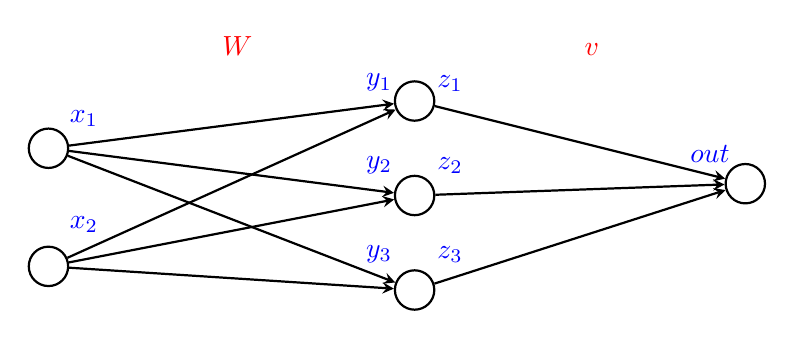
\begin{tikzpicture}[x=1.5cm, y=1.5cm, >=stealth]

        \foreach \m/\l [count=\y] in {1,2}
          \node [every neuron/.try, neuron \m/.try] (input-\m) at (-0.1,2.6-\y) {};
        
        \foreach \m [count=\y] in {1,2,3}
          \node [every neuron/.try, neuron \m/.try ] (hidden1-\m) at (3,2.8-\y*0.8) {};
        
        \foreach \m [count=\y] in {1}
          \node [every neuron/.try, neuron \m/.try ] (output-\m) at (5.8,2.3-\y) {};
        
        %\foreach \l [count=\i] in {1,2} 
        %  \draw [<-,thick] (input-\i) -- ++(-0.7,0)
         %   node [above, midway] {\scriptsize$x_\l$};
        
        %\draw [->,thick] (output-1) -- ++(0.7,0)
        %    node [above, midway] {\scriptsize$y$};

        \foreach \i in {1,...,2}
          \foreach \j in {1,...,3}
            \draw [->,thick] (input-\i) -- (hidden1-\j);

        \foreach \j in {1,...,3}
            \draw [->,thick] (hidden1-\j) -- (output-1);

       % \draw [->,thick] (input-1) -- (hidden1-1)
       %   node [above, midway] {\scriptsize$l_{21} = 1 - x_1~~$};
        %\draw [->,thick] (input-1) -- (hidden1-2)
        %  node [above, midway] {\scriptsize$l_{11} = x_1$};
        %\draw [->,thick] (input-2) -- (hidden1-3)
        %  node [above, midway] {\scriptsize$l_{12} = 1 - x_2$};
     %   \draw [->,thick] (input-2) -- (hidden1-4)
     %     node [above, midway] {\scriptsize$~~l_{22} = x_2$};
     %   \draw [->,thick] (input-3) -- (hidden1-5)
     %     node [above, midway] {\scriptsize$l_{13} = x_3$};
     %   \draw [->,thick] (input-4) -- (hidden1-6)
     %     node [above, midway] {\scriptsize$l_{23} = x_4$};
        
     %   \foreach \i in {1,4,6}
     %     \draw [->,thick] (hidden1-\i) -- (hidden2-2);

     %   \foreach \i in {2,3,5}
     %     \draw [->,thick] (hidden1-\i) -- (hidden2-1);
        %\foreach \l [count=\i] in {1,n}
        %  \node [above] at (hidden-\i.north) {$H_\l$};
        
        %\foreach \l [count=\i] in {1,n}
        %  \draw [->,thick] (output-\i) -- ++(1,0)
        %    node [above, midway] {$O_\l$};
        
        %\foreach \i in {1,...,4}
        %  \foreach \j in {1,...,2}
        %    \draw [->,thick] (input-\i) -- (hidden1-\j);
        
      %  \foreach \i in {1,...,2}
      %    \foreach \j in {1,...,2}
      %      \draw [->,thick] (hidden2-\i) -- (output-1);
        
        %\foreach \l [count=\x from 1] in {Input, Hidden, Ouput}
        %  \node [align=center, above] at (1+\x*2,2.6) {$\act_\x$};

        \node [align=center, above, color=blue] at (0.2, 1.7) {$x_1$};

        \node [align=center, above, color=blue] at (0.2, 0.8) {$x_2$};

        \node [align=center, above, color=blue] at (2.7, 1.3) {$y_2$};

        \node [align=center, above, color=blue] at (2.7, 2.0) {$y_1$};

        \node [align=center, above, color=blue] at (2.7, 0.55) {$y_3$};

        \node [align=center, above, color=blue] at (3.3, 1.3) {$z_2$};

        \node [align=center, above, color=blue] at (3.3, 2.0) {$z_1$};

        \node [align=center, above, color=blue] at (3.3, 0.55) {$z_3$};

        \node [align=center, above, color=blue] at (5.5, 1.4) {$out$};

        \node [align=center, above, color=red] at (1.5, 2.3) {$W$};
        \node [align=center, above, color=red] at (4.5, 2.3) {$v$};
        \node [align=center, above, color=red] at (3, 2.3) {$\act$};
        %\node [align=center, above] at (7, 2.5) {$\act_3$};
        
        %\node [align=center, above] at (5, 1.3) {\scriptsize$c_1=\act_2(\act_1(l_{11})+\act_1(l_{12})+\act_1(l_{13}))$};
        
        %\node [align=center, below] at (5, -1.3) {\scriptsize$c_2=\act_2(\act_1(l_{21})+\act_1(l_{22})+\act_1(l_{23}))$};
        
        %\node [align=center, below] at (7, -0.2) {\scriptsize$y = \act_3(c_1+c_2)$};
        \end{tikzpicture}
        \caption{A two-layer network example: 
$f(x) = v\act(Wx+b)+c$. We use the symbol $x$ to denote the input of the network, $y$ for the input of the hidden layer, $z$ for the output of the hidden layer, and $out$ as the out symbol. The subscript denotes the component within each symbol.}\label{fig:network}
        %\vspace{-1em}
     
\end{figure}

(\textbf{i}). The first interpretation is based on the observation that $\relu$'s slope is always within $[0,1]$, i.e., for any two inputs $y$ and $\Tilde{y}$ with $z = \relu(y)$ and $\Tilde{z} = \relu(\Tilde{y})$:
\[0 \leq \frac{z-\Tilde{z}}{y-\Tilde{y}}\leq 1.\]
This can be encoded with a quadratic relation: $((z-\Tilde{z})-(y-\Tilde{y}))(z-\Tilde{z})\leq 0$. This ReLU interpretation is used in~\cite{lipsdp}, and was named as the \emph{slope-restricted} activation. See~\cref{fig:relu} for an example. 

(\textbf{ii}). The second interpretation is from~\cite{sdp_rob_local}. $\relu$'s computation can be captured by the following three quadratic inequalities: $y\leq z$, $z\geq 0$ and $(z-y)z \leq 0$. One can easily verify that this encodes the computation of $\relu$ exactly. %We refer to this interpretation as the \emph{faithful} interpretation of $\relu$.

\begin{remark} 
It is to see that the slope-restricted interpretation is not unique to $\relu$, i.e., any function whose slope/derivative is between $0$ and $1$ has the same interpretation as $\relu$.
\end{remark}

\begin{remark}\label{rm:unique} 
The precise quadratic interpretation of $\relu$ is not unique. For example, we can introduce a new symbol $s$ to denote which branch of $\relu$ the execution is on. To express $\relu$'s computation, we can use $s(s-1) = 0$, $(s-1/2)y\geq 0$ and $z=sy$. This interpretation is similar to the one in~\cite{chen2020semialgebraic}. From this interpretation, one can view the slope-restricted interpretation as a \emph{stateless} interpretation of $\relu$, which does not consider the execution status of $y$.
\end{remark}
We also provide quadratic encodings for some other activation functions in~\cref{sec:other-act}. In particular, for those non-algebraic activation functions, we can use results from approximation theory to handle them.

\paragraph{Input perturbation}
Commonly considered attacks on the input are $\ell_2$ and $\ell_\infty$-attacks. Here we present how to encode them using quadratic relations. For other $\ell_p$-perturbations, we show their encodings in~\cref{sec:ell-p}.
Suppose that we have two inputs $x, \Tilde{x}\in \R^m$, if their $\ell_2$-distance is within $\epsilon$, then we can write it as:
\[
\sum_{i=1}^m (x_i-\Tilde{x}_i)^2 \leq \epsilon^2.
\]
If the $\ell_\infty$-distance between $x$ and $\Tilde{x}$ is within $\epsilon$, then $\max_i|x_i-\Tilde{x}_i|\leq \epsilon$. This can be encoded as $(x_i-\Tilde{x}_i)^2\leq \epsilon^2$ for all $i\in [m]$.

%We provide the quadratic encoding for general $\ell_p$ perturbations in \todo{cite}.

\subsection{Data-dependent Analysis}\label{sec:dept}
For data-dependent analysis, or local analysis, we fix an input $a\in \R^m$. We want to quantify the change of $f(a)$ if an $\ell_p$-perturbation with radius $\epsilon$ is added to the input. As a result, the quadratic program for the problem is:
\begin{subequations}
\begin{align}
    \max &\;vz+c \label{eq:obj}\\ 
    s.t.\;\;\;\;  & z_i(z_i-y_i)\leq 0, \;z_i\geq y_i, \;z_i\geq 0, \;\forall i\in [n]  \;\;(\relu \text{ computation}) \label{eq:relu}\\
    &y_i = w_i x+b_i,\;\forall i\in [n] \label{eq:first-layer}\\
    &\norm{x-a}_p\leq \epsilon \label{eq:pert}.
\end{align}
\end{subequations}
%$x$ denotes the input of $f$, $y$ denotes the input of the hidden layer, $z$ denotes the output of the hidden layer and the output of $f$ is the affine transformation of $z$.
The semantics of the symbols are the same as in~\cref{fig:network}. \Cref{eq:pert} denotes that $x$ is within the $\ell_p$-ball centered at $a$ with radius $\epsilon$. \Cref{eq:first-layer} denotes the affine transformation of the first layer, which constrains $x$ and $y$.  \Cref{eq:relu} denotes the element-wise computation of the $\relu$ hidden layer, which constrains $y$ and $z$. \Cref{eq:obj} is the objective that quantifies the output change. Because each equation exactly expresses the corresponding computation, this QP precisely encodes the verification problem of interest.

Now we demonstrate how to relax the quadratic program for $\ell_2$-perturbations using Shor's relaxation. The SDP for $\ell_\infty$-perturbations can be found in~\cite{sdp_rob_local}. The $\ell_2$-ball centered at $a$ can be expressed as
$\sum_{i=1}^m (x_i-a_i)^2\leq \epsilon^2$.
To relax the quadratic program to an SDP in the primal form, we first define a PSD variable $V\succeq 0$ with the decomposition as:
\[
V = \begin{pmatrix}
1 \;\;& z \;\;& x \\
z^T \;\;& Z \;\;& Y \\
x^T \;\;& Y^T \;\;& X \\
\end{pmatrix}
\]
Because $V$ is PSD, then $\exists M\in \R^{l\times (1+n+m)}$ for some $l\in\Z_+$ such that $V = M^TM$. Let us write $M = \begin{pmatrix}
u\;\; \bar{z}\;\; \bar{x}
\end{pmatrix}$ with $u^Tu = 1$. We can think of $u$, $\bar{z}$ and $\bar{x}$ as the multi-dimensional relaxations of $1$, $z$ and $x$. Representing the variables in $V$ with $M$'s components, we have $z = u^T\bar{z}$, $Z = \bar{z}^T\bar{z}$, $x = u^T\bar{x}$, $X= \bar{x}^T\bar{x}$, and $Y = \bar{z}^T\bar{x}$.

Because $y_i = w_ix+b_i$, we can substitute $y_i$ with $w_ix+b_i$. Now we are ready to present the SDP:
\begin{align}\label{eq:l2-cert-sdp}
\begin{split}
    \max &\;v z+c \\ 
    s.t.\;\;\;\;  & Z_{ii} - b_iz_i - w_iY_i^T \leq 0, \;z_i\geq w_ix+b_i, \;z_i\geq 0, \;\forall i\in [n] \\
    & \trace{(X)} - 2 x^T a + a^Ta - \epsilon^2\leq 0,%\\
    %&V\succeq 0, V_{11}=1
\end{split}
\end{align}
where $Y_i$ is the $i$-th row of $Y$.


For multi-layer networks, to construct the QP that expresses the verification problem, we only need to introduce more symbols to denote the input and output of the layers, and then constrain them using the quadratic relations as in the two-layer DNN case. It is then straightforward to relax the QP to SDP using Shor's relaxation. %suppose there are $d$-hidden layers, each of which has $n_j$ $\relu$ nodes. Let $W^j$ be the weight matrix between the $j$-th layer and the $(j+1)$-th layer, $b^j$ be the bias term, $w^j_i$ be the $i$-th row of $W^j$, and $v$ be the weight between $d$-th hidden layer and the output. We use $y^j$ to denote the inputs of the $j$-th hidden layer and $z^j$ be the output of the $j$-th hidden layer. Therefore, the QP for verifying the network is:
%\begin{align}\label{eq:multi-qp}
%\begin{split}
%    \max &\;vz^d+b^{d+1} \\ 
%    s.t.\;\;\;\;  & z^j_i(z^j_i-y^j_i)\leq 0, \;z^j_i\geq y^j_i, \;z^j_i\geq 0, \;\forall i\in [n_j], j\in [d] \\
%    &y^j_i = w^j_i z^{j-1}+b^j_i,\;\forall i\in [n_j], j\in \{2,\ldots,d\} \\
%    &y^1_i = w^1_i x+b^1_i,\;\forall i\in [n_1] \\
%    &\norm{x-a}_p\leq \epsilon
%\end{split}
%\end{align}
%To relax this program to an SDP, we only need to declare a PSD variable of size $(1+m+\sum_{i=1}^d n_i)\times (1+m+\sum_{i=1}^d n_i)$, and encode the objective and constraints in~\cref{eq:multi-qp} using the PSD variable.

\subsection{Data-independent Analysis}\label{sec:indept}
The data-independent analysis aims to quantify the change of a DNN, given a data-independent perturbation. In other words, we want to upper bound the change of the DNN output if a perturbation can be applied at any input point. This property is intrinsic to the neural network as a function, and not dependent on the data; and the problem is also known as the Lipschitz constant estimation of $f$. From mathematical analysis, the Lipschitz constant is the maximum operator norm over all possible gradients. %One can then consider an optimization program which
\cite{geolip} defined the formal global Lipschitz constant (FGL) as the maximum operator norm of all possible gradients, in which all the activation functions are considered independent. In reality, the activation functions are correlated and some of the activation patterns are infeasible. As a result, this value is a formal quantity and upper bounds the Lipschitz constant. \cite{geolip} indicated that most of the works on Lipschitz estimation and regularization, such as~\cite{alg-lip,lipsdp,gloro,certified_def} study the FGL instead of the Lipschitz constant. The study of FGL, especially the SDP estimation of this quantity~\cite{lipsdp}, inspires~\cite{alg-lip} to design $1$-Lipschitz network structures.

Using SDP to estimate the DNN Lipschitz constant was initiated by \cite{lipsdp}\footnote{\cite{certified_def} also devised an SDP to estimate the formal Lipschitz constant but the approach only works for two-layer networks.}, which only works for $\ell_2$-perturbations. \cite{lipopt} claimed that~\cite{lipsdp} could not transfer to the $\ell_\infty$ case. \cite{geolip} gave a compositional interpretation of~\cite{lipsdp} and generalized~\cite{lipsdp} to the $\ell_\infty$ case.
In fact, the SDPs for FGL estimation are just Shor's relaxation of QPs with the stateless $\relu$-interpretation. %; and pose an open question on the discrepancy between the FGL and the true Lipschitz constant. Here we show that not only the FGL can be estimated using the symbolic reasoning framework, but the true FGL can also be reasoned using the same framework. In fact, the difference is how we interpret the $\relu$ activation function.

\paragraph{Formal Lipschitzness estimation}
In FGL estimation, all activation are considered independent, therefore, one does not need to consider the actual execution state of the $\relu$ function. \cite{geolip} used $\Delta x$ to denote the difference between two inputs $x$ and $\Tilde{x}$, and similarly $\Delta y$ for $y$ and $\Tilde{y}$, $\Delta z$ for $z$ and $\Tilde{z}$. The following QP can encode the FGL-estimation problem:
\begin{align}\label{eq:formal}
\begin{split}
  \max &\;v\Delta z \\ 
    s.t.\;\;\;\;  & (\Delta z_i - \Delta y_i)\Delta z_i\leq 0, \;\forall i\in [n] \\
    & \Delta y_i = w_i \Delta x,\;\forall i\in [n]\\
    &\norm{\Delta x}_p\leq 1  .
\end{split}  
\end{align}
An interpretation of this program is to quantify how a data-independent perturbation $\Delta x$ propagates from the input layer to the output layer. The propagation is subject to the $\ell_p$-norm and DNN computation constraints.
\cite{geolip} provided more details on the relaxed SDPs of~\cref{eq:formal}, the relations to the mixed-norm problem and the Grothendieck inequalities~\cite{cut-norm,GroIneq,nest}. In particular, the SDPs in \cite{lipsdp} and~\cite{certified_def} are just Shor's relaxations of~\cref{eq:formal} within their application scope in the primal and dual forms.

